\chapter{Approche}

\epigraph{<< Les plans sont inutiles, mais la planification est indispensable >>}{Dwight David Eisenhower}

\section{Méthodologie}
% Parler de notre façon de fonctionner : SUPER AGILE !

De part la nature ouverte du projet à accueillir continuellement des nouvelles fonctionnalités et changements, une méthode Agile a été plébiscitée (qui s'opposent aux méthodes classiques plus rigides comme \textit{waterfall}). Comme expliqué par le manifeste Agile\cite{agileManifeste}, un certain nombre de principes sont présents et nous n'évoquerons ici que les plus importants : 

\begin{description}
    \item[\textbf{Satisfaction du client avant tout}] Il s'agit du principe sacro-saint de la méthode Agile\cite{agileManifeste}. Au lieu d'avoir un planning bien ficelé, il faut accepter l'ajout de nouvelles fonctionnalités et des changements (même tardifs) pour viser ce but.
    
    \item[\textbf{Itérations courtes}] En méthode Agile\cite{agileManifeste}, il est préconisé d'adopter des cycles de développement de faible durée afin de notamment identifier et corriger très tôt des bugs (une expression anglophone y est dédiée : "fail fast, fail often"). Puisque nous rencontrions nos promoteurs à peu près toutes les semaines, c'est naturellement ce rythme qui s'est imposé pour nos itérations.
    
    \item[\textbf{Livraison continue}] Tout au long du projet, de nombreux utilisateurs dont nos promoteurs ont utilisé intensivement l'application et nous ont livré quantité d'avis et retours. Il était donc nécessaire de déployer des versions de l'application très régulièrement pour montrer son avancement et donner la possibilité d'essayer de nouvelles fonctionnalités par les utilisateurs : nous avons fini par automatiser une grande partie de ce processus (nous expliquerons en détail dans la section TODO comment cela a été réalisé concrètement).
\end{description}

\subsection*{Phases du mémoire}

% Expliquer les différentes types de phase par lesquelles on est passé
% - Analyse
% - Architecture
% - Implémentation
% - Validation
% - Testing
% - Rédaction
% - Version alpha en décembre
% - ...

Pouvoir baliser les grandes étapes de ce travail est nécessaire  
%TODO %
\\ TODO

% une section sur la communication
\subsection*{Communication}

En méthode Agile\cite{agileManifeste}, il y a de manière générale 2 questions récurrentes, et ce peu importe la taille et la nature des projets :
\begin{itemize}
    \item Où on en est ? 
    \begin{itemize}
        \item À quelle vitesse on progresse ?
        \item Qu'avons nous réalisé ?
    \end{itemize}
    \item Quand on délivre le produit ?
    \begin{itemize}
        \item Que reste il à faire ?
        \item Comment estimer le temps/travail nécessaire pour réaliser les différentes tâches ?
    \end{itemize}
\end{itemize}

Pour y répondre, il convient d'utiliser des moyens/outils de communication suffisamment explicites. Étant donné que notre solution est hébergé sur Github, nous avons décidé d'utiliser les fonctionnalités suivantes de Github : le "Project Board" \footnote{\url{https://help.github.com/en/github/managing-your-work-on-github/about-project-boards}} et les issues \footnote{\url{https://help.github.com/en/github/managing-your-work-on-github/about-issues}}. (dont vous pourrez trouver une illustration respectivement aux figures \ref{pic:GithubBoard} et \ref{pic:GithubIssues} )\\

Comme nous pouvons le voir, par l'usage des ces outils/moyens, l'état et la progression générale du projet sont accessibles au plus grand nombre : 
\begin{itemize}
    \item Avec le "Project Board", on représente les tâches sous la forme de cartes amovibles dans un tableau, avec les caractéristiques suivantes :
    \begin{itemize}
        \item Chaque tâche est catégorisée dans une colonne bien précise ( "to do"/ à réaliser, "in progress"/ en cours, "done" / réalisée, "enhancements" / améliorations  )
        \item Une barre de progression nous notifie de l'avancement générale du projet
    \end{itemize}
    \item Avec les issues (figure \ref{pic:GithubIssues}), chaque tâche/problème dispose des éléments suivants : 
    \begin{itemize}
        \item un titre pour expliquer brièvement celle-ci
        \item une étiquette en couleur pour notifier sa nature (problème, amélioration, documentation, etc)
        \item la personne assignée sur celle-ci
        \item le statut de celle-ci (ouverte/fermée)
    \end{itemize}
\end{itemize}


% width=\textwidth,height=\textheight,keepaspectratio
\begin{figure}[H]
    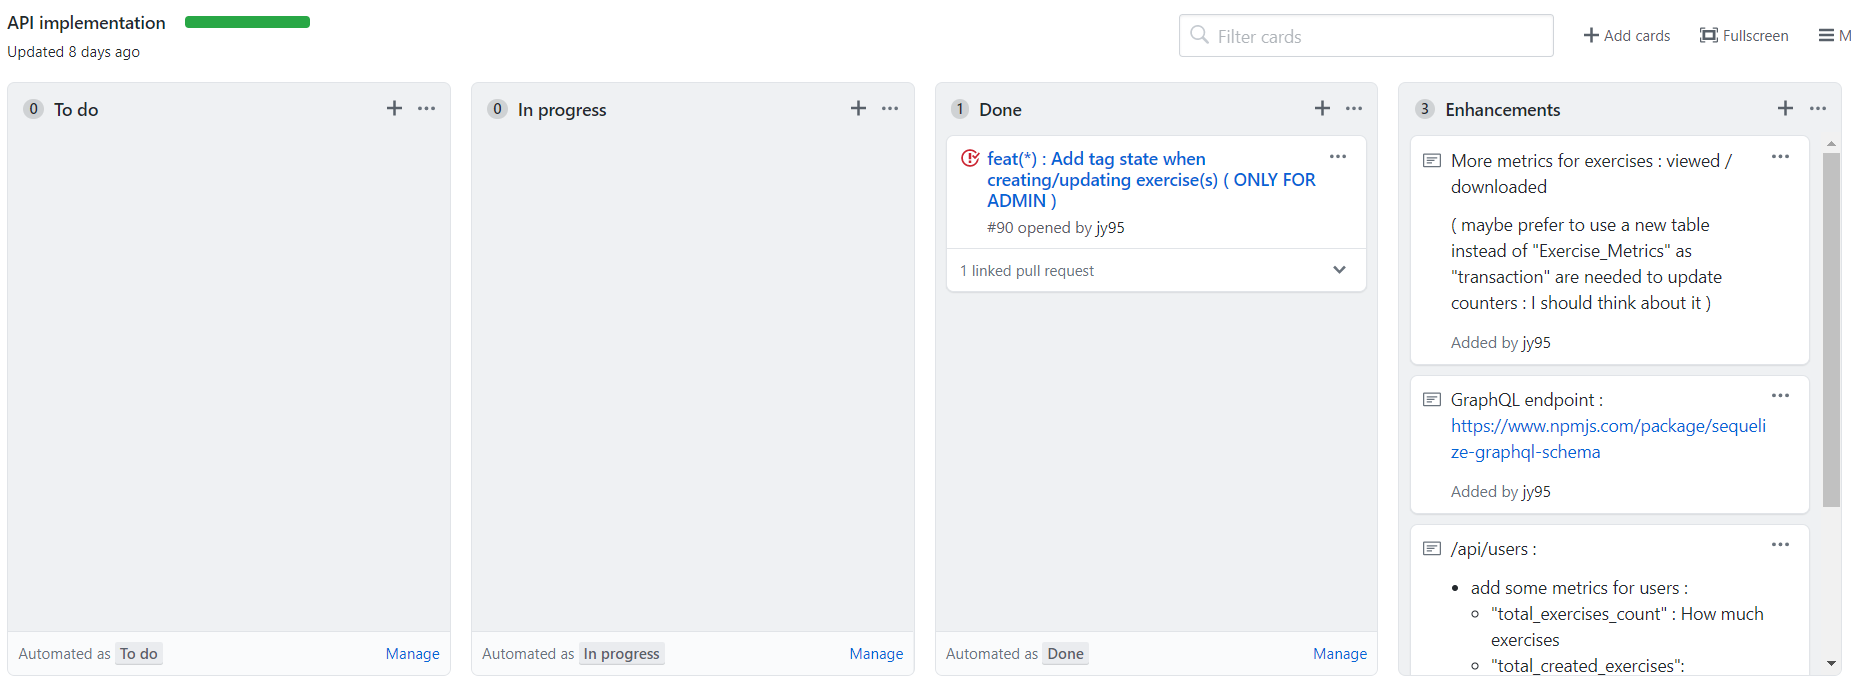
\includegraphics[width=\textwidth,height=\textheight,keepaspectratio]{images/trelloLike.PNG}
    \centering
    \caption{Exemple simplifié d'interface Github Project Board}
    \label{pic:GithubBoard}
\end{figure}

% width=\textwidth,height=\textheight,keepaspectratio
\begin{figure}[H]
    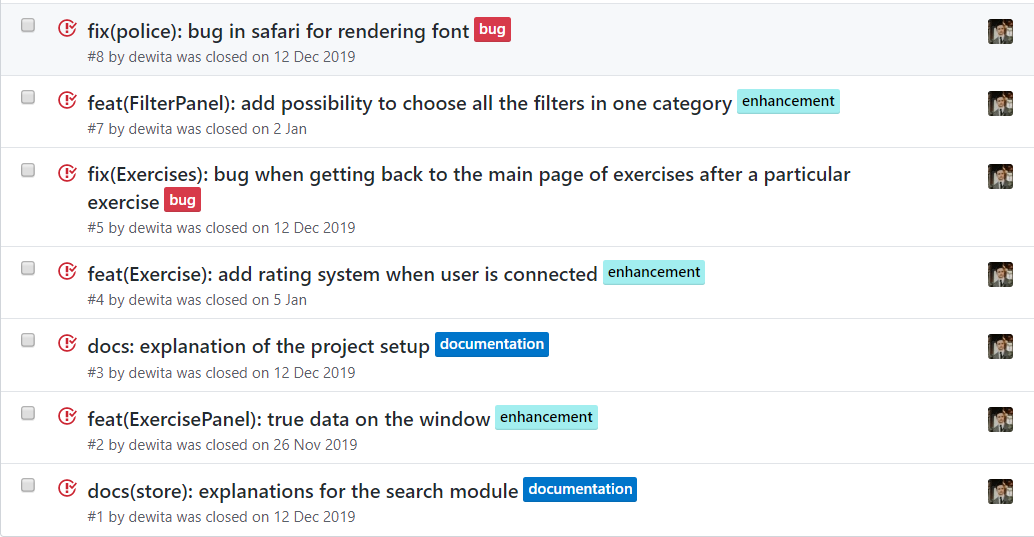
\includegraphics[width=\textwidth,height=\textheight,keepaspectratio]{images/issueList.PNG}
    \centering
    \caption{Exemple simplifié d'issues sur Github}
    \label{pic:GithubIssues}
\end{figure}

\section{Planning}
% Une illustration résumée est appréciable à un millier de mots ^^
\section{Organisation du travail}
% Backend
% Front
% + les différentes phases du mémoire